\documentclass[a4paper,12pt]{book} % nie: report!


% pakiety
\usepackage{polski} % lepiej to zamiast babel!
\usepackage[utf8]{inputenc} % w razie kłopotów spróbować: \usepackage[utf8x]{inputenc}
\usepackage{fancyhdr} % nagłówki i stopki
\usepackage{indentfirst} % WAŻNE, MA BYĆ!
\usepackage[pdftex]{graphicx} % to do wstawiania rysunków
\usepackage{amsmath} % to do dodatkowych symboli, przydatne
\usepackage[pdftex,
            left=1in,right=1in,
            top=1in,bottom=1in]{geometry} % marginsy
\usepackage{amssymb} % to też do dodatkowych symboli, też przydatne
\usepackage{pdfpages}
\usepackage{lipsum}
\usepackage{multirow}
\usepackage{listings}

% definicje nagłówków i stopek
\pagestyle{fancy}
\renewcommand{\chaptermark}[1]{\markboth{#1}{}}
\renewcommand{\sectionmark}[1]{\markright{\thesection\ #1}}
\fancyhf{}
\fancyhead[LE,RO]{\footnotesize\bfseries\thepage}
\fancyhead[LO]{\footnotesize\rightmark}
\fancyhead[RE]{\footnotesize\leftmark}
\renewcommand{\headrulewidth}{0.5pt}
\renewcommand{\footrulewidth}{0pt}
\addtolength{\headheight}{1.5pt}
\fancypagestyle{plain}{\fancyhead{}\cfoot{\footnotesize\bfseries\thepage}\renewcommand{\headrulewidth}{0pt}}


% interlinia
\linespread{1.25}


% treść
\begin{document}
\sloppy



\thispagestyle{empty}


\includepdf{stronatytulowa}
% najpierw uzupełnij w 'stronatytulowa.odt' openoffice i wyeksportuj do 'stronatytulowa.pdf'

\newpage{}

\thispagestyle{empty}

\newpage{}



\tableofcontents{}

\chapter{}
\section{Wstęp}
\label{Wstep}
%Mega ogólne sprawy dotyczące tego co chce zrobić
\lipsum[1]

\section{Cel i teza pracy}
\label{Cel i teza pracy}
%celem pracy jest napisanie programu bla bla
\lipsum[1]

\section{Zakres pracy}
\label{Zakres pracy}
%Trza zrobic research bla bla
\begin{itemize}
	\item Przegląd metod analizy obrazu;
	\item Przegląd dostępnych sieci neuronowych dedykowanych do analizy obrazu;
	\item Opracowanie specyfikacji sprzętowej niezbędnej do realizacji prototypowego systemu;
	\item Wytworzenie oprogramowania realizującego wykrywanie łuku elektrycznego;
	\item Analiza wyników i szybkości działania zastosowanych metod YoLo, R-CNN;
\end{itemize}
\lipsum[1]

\chapter{Rozdział o czymś tam}

\section{Sekcja A}

\begin{figure}[h]
	\centering
	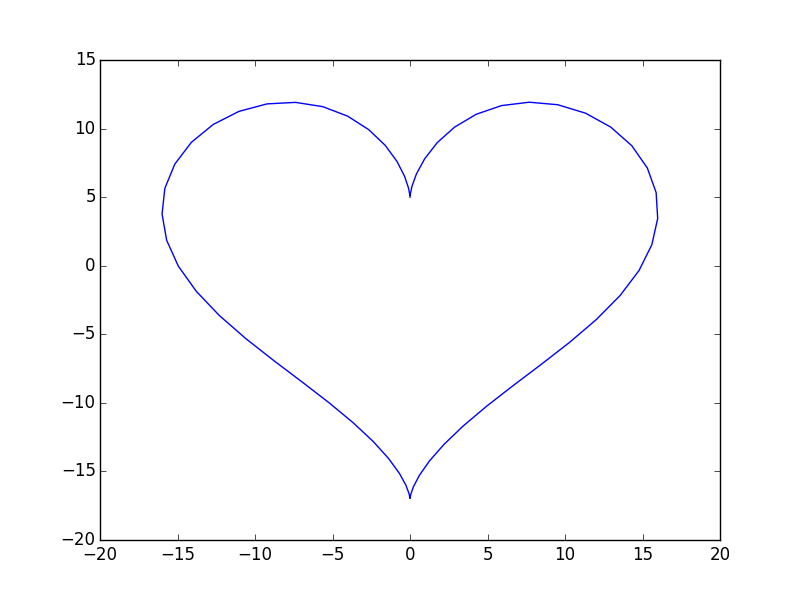
\includegraphics[width=14cm]{figures/heart.png}
	\caption{Serduszko}
	\label{fig1}
\end{figure}


\section{Sekcja B}

\begin{table}[h]
	\centering
	\caption{Wino}
	\begin{tabular}{lcccllll}
		\multicolumn{1}{c}{{\color[HTML]{44546A} }} &
		{\color[HTML]{44546A} } &
		{\color[HTML]{44546A} } &
		{\color[HTML]{44546A} } &
		\multicolumn{1}{c}{{\color[HTML]{44546A} }} &
		\multicolumn{1}{c}{{\color[HTML]{44546A} }} &
		\multicolumn{2}{c}{{\color[HTML]{44546A} \textbf{Partia przed burzliwą}}} \\
		\multicolumn{1}{c}{\multirow{-2}{*}{{\color[HTML]{44546A} \textbf{Oczekiwany typ wina}}}} &
		\multirow{-2}{*}{{\color[HTML]{44546A} \textbf{Data nastawu}}} &
		\multirow{-2}{*}{{\color[HTML]{44546A} \textbf{Data zastawienia fermentacji cichej}}} &
		\multirow{-2}{*}{{\color[HTML]{44546A} \textbf{Data zlania do butelek}}} &
		\multicolumn{1}{c}{\multirow{-2}{*}{{\color[HTML]{44546A} \textbf{Ilość moszczu {[}kg{]}}}}} &
		\multicolumn{1}{c}{\multirow{-2}{*}{{\color[HTML]{44546A} \textbf{Zabezpieczenie   pirosiarczanem potasu {[}g{]}}}}} &
		{\color[HTML]{44546A} \textbf{Woda   {[}L{]}}} &
		{\color[HTML]{44546A} \textbf{Cukier {[}kg{]}}} \\
		Czerwone słodkie/półsłodkie MEŁGIEW &
		16.10.2021 &
		24.10.2021 &
		\multicolumn{1}{l}{} &
		15,660 &
		1,566 &
		3,132 &
		3,132 \\
		Czerwone słodkie/półsłodkie BIŁGORAJ 1/2 &
		&
		&
		&
		15,000 &
		1,500 &
		3,000 &
		3,000 \\
		Czerwone słodkie/półsłodkie BIŁGORAJ 2/2 &
		\multirow{-2}{*}{27.10.2021} &
		\multirow{-2}{*}{05.11.2021} &
		\multirow{-2}{*}{} &
		10,000 &
		1,000 &
		2,000 &
		2,000
	\end{tabular}
\end{table}


\chapter{Rozdział o czymś innym}

\section{Sekcja C}


\section{Sekcja D}


\listoftables{} % jeśli są tabele
\addcontentsline{toc}{chapter}{Spis tabel}

\listoffigures{} % jeśli są tabele
\addcontentsline{toc}{chapter}{Spis rysunków}

\addcontentsline{toc}{chapter}{Bibliografia}
\bibliographystyle{ieeetr}
\bibliography{bibliography/yolo}


\end{document}
